%%
%% Copyright 2007, 2008, 2009 Elsevier Ltd
%%
%% This file is part of the 'Elsarticle Bundle'.
%% ---------------------------------------------
%%
%% It may be distributed under the conditions of the LaTeX Project Public
%% License, either version 1.2 of this license or (at your option) any
%% later version.  The latest version of this license is in
%%    http://www.latex-project.org/lppl.txt
%% and version 1.2 or later is part of all distributions of LaTeX
%% version 1999/12/01 or later.
%%
%% The list of all files belonging to the 'Elsarticle Bundle' is
%% given in the file `manifest.txt'.
%%

%% Template article for Elsevier's document class `elsarticle'
%% with harvard style bibliographic references
%% SP 2008/03/01
%%
%%
%%
%% $Id: elsarticle-template-harv.tex 4 2009-10-24 08:22:58Z rishi $
%%
%%
%%\documentclass[preprint,authoryear,12pt]{elsarticle}

%% Use the option review to obtain double line spacing
\documentclass[authoryear,preprint,review,12pt]{elsarticle}

%% Use the options 1p,twocolumn; 3p; 3p,twocolumn; 5p; or 5p,twocolumn
%% for a journal layout:
%% \documentclass[final,authoryear,1p,times]{elsarticle}
%% \documentclass[final,authoryear,1p,times,twocolumn]{elsarticle}
%% \documentclass[final,authoryear,3p,times]{elsarticle}
%% \documentclass[final,authoryear,3p,times,twocolumn]{elsarticle}
%% \documentclass[final,authoryear,5p,times]{elsarticle}
%% \documentclass[final,authoryear,5p,times,twocolumn]{elsarticle}

%% if you use PostScript figures in your article
%% use the graphics package for simple commands
\usepackage{graphics}
\usepackage{longtable}
%% or use the graphicx package for more complicated commands
%% \usepackage{graphicx}
%% or use the epsfig package if you prefer to use the old commands
%% \usepackage{epsfig}

%% The amssymb package provides various useful mathematical symbols
\usepackage{amssymb}
%% The amsthm package provides extended theorem environments
\usepackage{amsthm}
\usepackage{colortbl}

%% The lineno packages adds line numbers. Start line numbering with
%% \begin{linenumbers}, end it with \end{linenumbers}. Or switch it on
%% for the whole article with \linenumbers after \end{frontmatter}.
%% \usepackage{lineno}

%% natbib.sty is loaded by default. However, natbib options can be
%% provided with \biboptions{...} command. Following options are
%% valid:

%%   round  -  round parentheses are used (default)
%%   square -  square brackets are used   [option]
%%   curly  -  curly braces are used      {option}
%%   angle  -  angle brackets are used    <option>
%%   semicolon  -  multiple citations separated by semi-colon (default)
%%   colon  - same as semicolon, an earlier confusion
%%   comma  -  separated by comma
%%   authoryear - selects author-year citations (default)
%%   numbers-  selects numerical citations
%%   super  -  numerical citations as superscripts
%%   sort   -  sorts multiple citations according to order in ref. list
%%   sort&compress   -  like sort, but also compresses numerical citations
%%   compress - compresses without sorting
%%   longnamesfirst  -  makes first citation full author list
%%
%% \biboptions{longnamesfirst,comma}

% \biboptions{}

\journal{Expert Systems with Applications}

\newtheorem{definition}{Definition}
\newtheorem{proposition}{Proposition}

\begin{document}

\begin{frontmatter}

%% Title, authors and addresses

%% use the tnoteref command within \title for footnotes;
%% use the tnotetext command for the associated footnote;
%% use the fnref command within \author or \address for footnotes;
%% use the fntext command for the associated footnote;
%% use the corref command within \author for corresponding author footnotes;
%% use the cortext command for the associated footnote;
%% use the ead command for the email address,
%% and the form \ead[url] for the home page:
%%
%% \title{Title\tnoteref{label1}}
%% \tnotetext[label1]{}
%% \author{Name\corref{cor1}\fnref{label2}}
%% \ead{email address}
%% \ead[url]{home page}
%% \fntext[label2]{}
%% \cortext[cor1]{}
%% \address{Address\fnref{label3}}
%% \fntext[label3]{}

\title{Hardware Platform for Computing Irreducible Testors Based on CT-EXT}

%% use optional labels to link authors explicitly to addresses:
%% \author[label1,label2]{<author name>}
%% \address[label1]{<address>}
%% \address[label2]{<address>}


\address{Computer Science Department}
\address{National Institute for Astrophysics, Optics and Electronics}
\address{Sta. Ma. Tonanzintla, Puebla, 72840, Mexico}

\begin{abstract}
Feature selection is an important task in pattern recognition. Given a dataset described by a set of attributes, a minimum subset of attributes that preserves the ability to discern between objects from different classes is needed. The computation of this minimum subset is a problem whose space complexity increases
exponentially regarding the number of attributes. The Testor theory is a convenient way to solve this problem. A testor is defined as a subset of attributes that can discern between objects of different classes; and a typical testor is a minimal subset with this property. Although there are efficient algorithms for computing typical testors, hardware implementations of these algorithms can improve their performance; taking advantage of the inherent parallelism in the evaluation of testor candidates. In this paper a hardware platform based on an efficient algorithm for computing irreducible testors for feature selection in pattern recognition is presented. Results from a prototype implementation on an FPGA board, showing the advantages of the proposed platform, are presented and discussed.

%In pattern recognition, feature selection is a very important task
%for supervised classification. The problem consists in, given a
%dataset where each object is described by a set of features, finding
%a subset of the original features such that a classifier that runs
%on data containing only these features would reach high
%classification accuracy. A useful way to find this subset of the
%original features is through Testor Theory. A testor is defined as a
%subset of the original features that allows differentiating objects
%from different classes. Testors are very useful particularly when
%object descriptions contain both numeric and non-numeric features.
%Computing testors for feature selection is a very complex problem
%due to exponential complexity, with respect to the number of
%features, of algorithms based on testor theory. Hardware
%implementation of testor computing algorithms helps to improve their
%performance taking advantage of parallel processing for verifying if
%a feature subset is a testor in a single clock cycle. This paper
%introduces an efficient hardware-software platform for computing
%irreducible testors for feature selection in pattern recognition.
%Results of implementing the proposed platform using a FPGA-based
%prototyping board are presented and discussed.

\end{abstract}

\begin{keyword}
%% keywords here, in the form: keyword \sep keyword
Feature Selection \sep Testor Theory \sep Custom Architectures \sep
FPGAs
%% MSC codes here, in the form: \MSC code \sep code
%% or \MSC[2008] code \sep code (2000 is the default)

\end{keyword}

\end{frontmatter}

% \linenumbers

%% main text
\section{Introduction}
\label{sect:1}

%Reconfigurable computing based on the combination of conventional
%microprocessors and field programmable gate arrays (FPGAs), has
%become increasingly popular for implementing special-purpose
%hardware to accelerate complex tasks. Usually an FPGA-based
%implementation is embedded in a PC or workstation, which drives its
%activity and manages the results. 

Feature selection problem in supervised classification consists in identifying those attributes that 
provide relevant information for the classification process. This procedure does not only reduce the 
computational cost of classification process by eliminating superfluous information, but in some cases 
it can even provide better classification accuracy. Several algorithms have been proposed to overcome 
the exponential complexity intrinsic to feature selection, however, most of them were restricted to 
numeric attributes \citep{R3,R4}. Testor theory can be used for feature selection with mixed and incomplete 
data as shown in~\citep{R27,R5}. A testor is defined as a subset of attributes that can discern between 
objects of different classes. An irreducible testor is a subset in which every attribute is indispensable 
for satisfying testor condition. Finding all irreducible testors is a computationally complex problem.

Recently, there is an increasing popularity of FPGA-based architectures for solving complex 
computational problems. Several hardware-software platforms based on this technology have been 
reported \citep{R29,R30}. 
In these platforms, the software component handles those tasks less suited for hardware implementation, 
and is also responsible of configuring the FPGA, as well as handling communication with it. 
The hardware component, on the other hand, performs those operations with a high parallelism degree.

In spite of advances in the theoretical aspect of computing
irreducible testors \citep{R5,R8,R9}, there are 
no hardware implementations reported aside from \citep{R10,R11,R21}.
In the first work, an FPGA-based brute force approach for computing testors was proposed
\citep{R10}. This first approach didn't take advantage of dataset characteristics to reduce the number 
of candidates to be tested. Thus all $2^N$ combinations were tested. Then in \citep{R11} a hardware 
architecture of the BT algorithm for computing typical testors was implemented. 
This algorithm used a candidate pruning process that avoids unnecessary candidates evaluation, 
reducing the number of irreducible testors conditions verifications. 
These two previous works computed the whole set of testors on the FPGA device whilst irreducible condition 
was evaluated afterwards by the software component in the hosting PC. 
Thus \cite{R21} proposed a hardware-software platform for computing irreducible testors that 
implemented the BT algorithm, as in \citep{R11}, but it also included a new module that eliminates most of 
the non irreducible testors before transferring them to a host software application for final filtering. 
One disadvantage of these approaches is the huge amount of data to be transferred to the PC.  
Following this idea, we developed an efficient hardware-software platform for computing irreducible
testors for feature selection in pattern recognition \citep{R2,R3,R17,R18,R19} using 
CT-EXT, an algorithm based on testor theory, proposed in~\citep{R22}. CT-EXT has proven being, in most cases, 
more efficient in finding typical testors than the BT algorithm~\citep{R22, R23}.

The intensive computational requirements due to the exponential
complexity, with respect to the number of features, of the CT-EXT algorithm 
can be met by a combination of technological
improvements and efficient hardware architectures based on parallel
computational models. Further optimizations such as incremental
processing and the use of multiple processing elements are also
possible as will be shown later in this paper.

The rest of this paper is structured as follows. Section~\ref{sect:2} introduces the basic concepts of 
Testor theory and the CT-EXT algorithm. Section~\ref{sect:3} exposes the proposed platform. 
Section~\ref{sect:4} describes the hardware architecture. Section~\ref{sect:5} depicts the software component. 
Evaluation of proposed platform and discussion of experiments results are presented in sections~\ref{sect:6} 
and~\ref{sect:7}. Finally, section~\ref{sect:8} shows the most important conclusions.

\section{Basic concepts}
\label{sect:2}

In pattern recognition, feature selection is a very important task for supervised classification. In the logical
 combinatorial approach to pattern recognition \citep{R5}
%TODO include J. Ruiz-Shulcloper, M.A. Abidi. Logical Combinatorial Pattern Recognition: A Review // In S.G. Pandalai. Recent Research Developments in Pattern Recognition. 2002. P 133-76. 
 , a useful
way to deal with this problem is through Testor Theory. The concept of testor for pattern recognition was
introduced by Dmitriev et al. in 1966 \citep{R12}. They defined a testor as a subset of features that allows
differentiating objects from different classes. Testors are quite useful, especially when object descriptions
contain both numeric and non-numeric features, and maybe they are incomplete (mixed incomplete data)
\citep{R5}.

Let $TM$ be a training matrix with $K$ objects described through $N$
features of any type $\{x_{1},\ldots,x_{N}\}$ and grouped in $r$
classes. Let $DM$ be a dissimilarity Boolean matrix (0 = similar,1 =
dissimilar), obtained from feature by feature comparisons of every
pair of objects from $TM$ belonging to different classes. $DM$ has
$N$ columns and $M$ rows, where $M>>K$.

Let $T$ be a subset of attributes. Testors and irreducible testors are formally defined as follows:

\begin{definition} \label{def1}
$T$ is a testor if and only if when all
features are eliminated from $DM$, except those from $T$, there is
not any row of $DM$ with only 0's. $T$ is an irreducible testor if none of its subsets is a testor.
\end{definition}

In defintion \ref{def1}, if there is not any row of $DM$ with only
0's it means that there is not a pair of objects from different
classes that are similar on all the features of $T$, that is, a
testor $T$ allows differentiating between objects from different
classes. From definition~\ref{def1}, if $T$ is a testor then, any superset of $T$ is a testor too.

The number of rows in $DM$ could be too large, therefore a strategy to reduce this matrix without losing
relevant information for computing irreducible testors was introduced by Lazo et al \citep{R1}.

%% DEFINICION 
\begin{definition}
Let $f=[f_1, f_2, \dots , f_n]$ and $f'=[f'_1, {f'}_2, \dots , {f'}_n]$ two rows of $DM$, we say that $f$ 
is a sub-row of $f^{'}$ if for each column $j=1,2,\dots ,n$;  $f_{j} \le f'_{j}$ and for at least one index the 
inequality is strict.
\end{definition}

%% DEFINICION 
\begin{definition}
We say that a row $f$ of $DM$ is a basic row if no row of the matrix $DM$ is a sub-row of $f$. 
\end{definition}

%% DEFINICION 
\begin{definition}
The sub-matrix of $DM$ formed only by the basic rows (without repetitions) is called basic matriz and is denoted by $BM$ .
\end{definition}

Let $TT(M)$ be the set of all irreducible testors of the Boolean matrix M, then following \citep{R21} we have 
that $TT(DM)=TT(BM)$; i.e., we can conclude that normally $DM$ contains redundant information. In addition, 
the construction of $BM$ from $DM$ is a very fast process, then we focus our work on $BM$.

%\section{Basic concepts}
%\label{sect:2}
%
%In pattern recognition, feature selection is a very important task for supervised classification. A useful
%way to do this selection is through Testor Theory. The concept of testor for pattern recognition was
%introduced by Dmitriev et al. in 1966 \citep{R12}. They defined a testor as a subset of features that allows
%differentiating objects from different classes. Testors are quite useful, especially when object descriptions
%contain both numeric and nonnumeric features, and maybe they are incomplete (mixed incomplete data)
%\citep{R5}.
%
%Let $TM$ be a training matrix with $K$ objects described through $N$
%features of any type $(x_{1},\ldots,x_{N})$ and grouped in $r$
%classes. Let $DM$ be a dissimilarity Boolean matrix (0 = similar,1 =
%dissimilar), obtained from feature by feature comparisons of every
%pair of objects from $TM$ belonging to different classes. $DM$ has
%$N$ columns and $M$ rows, where $M>>K$.
%
%Testors and irreducible testors are defined as follows:
%
%\begin{definition} \label{def1}
%A subset of features $T$ is a testor if and only if when all
%features are eliminated from $DM$, except those from $T$, there is
%not any row of $DM$ with only 0�s.
%\end{definition}
%
%
%\begin{definition} \label{def2}
%A subset of features $T$ is an irreducible testor if and only if $T$
%is a testor and there is not any other testor $T'$ such that
%$T'\subset T$.
%\end{definition}
%
%In defintion \ref{def1}, if there is not any row of $DM$ with only
%0's it means that there is not a pair of objects from different
%classes that are similar on all the features of $T$, that is, a
%testor $T$ allows differentiating between objects from different
%classes.
%
%The number of rows in $DM$ could be too large, therefore a strategy to reduce this matrix without losing
%relevant information for computing irreducible testors was introduced by Lazo et al \citep{R1}.
%
%\begin{definition} \label{def3}
%If $t$ and $p$ are two rows of $DM$, then $p$ is a sub-row of $t$ if and only if:
%
%
%\begin{enumerate}
%\renewcommand{\labelenumi}{\alph{enumi})}
%\item $t$ has 1 everywhere $p$ has 1
%\item there is at least one column such that $t$ has 1 and $p$ has 0
%\end{enumerate}
%\end{definition}
%
%\begin{definition} \label{def4}
%A row $t$ of $DM$ is a basic row of $DM$ if and only if $DM$ does
%not have any other row $t' $ such that $t' $ is a sub-row of $t$.
%\end{definition}
%
%\begin{definition} \label{def5}
%The matrix that contains only the basic rows of $DM$ is called basic
%matrix and is denoted by $BM$.
%\end{definition}
%
%Let $TT(M)$ be the set of all irreducible testors of the Boolean matrix M, then
%
%\begin{proposition}
%$TT(DM)=TT(BM)$.
%\end{proposition}
%
%This proposition indicates that the set of all irreducible testors calculated using $DM$ or $BM$ is the same
%\citep{R1}. However, $BM$ is smaller than $DM$ and the construction of $BM$ from $DM$ is a very fast process,
%for example, the time for obtaining a $BM$ matrix with 48 columns and 32 rows from a $DM$ matrix with 48
%columns and 193,753 rows, is about 0.21 seconds on a PC with an Intel Centrino Duo processor running at
%1.6GHz, with 1024 MB of RAM.

The CT-EXT has the following theoretical bases.
\begin{definition} \label{def21} Let $f_i$ be a row of BM. We say that $f_i$ is a zero row of $S \subseteq R$, and we denote it by ${f_i}^0 (S)$, if $\forall X_p \in S$, $f_i [p] = BM [i, p] = 0$.
\end{definition}
\begin{definition} \label{def22} In terms of BM, a testor $T \subseteq R$ is a feature set such that there
are no zero rows of T in BM. 
\end{definition}
\begin{definition} \label{def23} Let $f_i$ be a row of BM. We say that $f_i$ is a typical (irreducible) row of $S \subseteq R$ with regard to $X_q$, being $X_q \in S$, and we denote it by ${f_i}^1 (S,q)$ if $f_i [q] = BM [i, q] = 1$, and $\forall X_p \in S$, $X_p \neq X_q$ , $f_i [p] = BM [i, p] =~0$.
\end{definition}

\begin{definition} \label{def24} In terms of BM, $T \subseteq R$ is a typical testor if T is a testor and
$\forall X_j \in T, \exists {f_i}^1 (T, j)$.
\end{definition}

This means that for all features in a typical testor, there exists a row in $BM$ in
the sub matrix associated to $T$, having a 1 in the position corresponding
to that feature, and 0 in all remaining positions (there are no zero rows,
and if any column of $T$ is eliminated, at least one zero row will appear, and the testor
property will not be fulfilled). Although we have defined a typical testor here in terms
of $BM$, usually it is also defined in terms of $DM$ as an irreducible testor in definition~\ref{def1}.

\begin{definition} \label{def25} Let $T \subseteq R$ and $X_j \in R$, $X_j \notin T$. We denote by
$\sum_T f^0$ the number of zero rows of T. We say that $X_j$ contributes to T if, and only if,
$\sum_{T\cup\{X_j\}} f^0 < \sum_T f^0$.
\end{definition}
This definition indicates that one feature contributes to a feature combination
if for some zero rows in $BM$, considering only $T$, the new feature has a 1 in 
at least one of these zero rows. So, adding this feature to $T$, there are less
zero rows than the amount of zero rows for $T$.

Being $T \subset T\cup\{X_j\}$, it is not possible that $\sum_T f^0 < \sum_{T\cup\{X_j\}} f^0$. If we
increase the feature combination either the zero rows are maintained and in this
case the column added does not contribute to the combination, or the number of zero rows decreases.

Propositions~\ref{prop1} and~\ref{prop2} are important conclusions for CT-EXT which were introduced and 
proved in \citep{R22}.

\begin{proposition}\label{prop1} Let $T \subseteq R$ and  $X_j \in R$, $X_j \notin T$. If $X_j$ does not contribute to T, then $T\cup\{X_j\}$ can not generate any typical testor.
\end{proposition}

%\textit{Proof}. Let $T \subseteq R$ and $X_j \in R$, such that $X_j$ does not contribute to T. Suppose
%that $T' = T\cup\{X_j \cup Z\}$ is a typical testor. Then, according to definition \ref{def24}, there
%exists for $X_j$ at least a typical row in $BM$. Then, $f_i [j] = BM [i, j] = 1$, and
%$\forall X_p \in T'$ , $X_p \neq X_j$ , $f_i [p] = BM [i, p] = 0$. Thus, we have that $f_i$ is a zero row
%of $T \cup Z$ and therefore, it is also a zero row of $T$. So, $\sum_{T\cup\{X_j\}} f^0 < \sum_T f^0$ and we obtain that
%$X_j$ contributes to $T$, which contradicts the formulated hypothesis and then, we
%have that there are no typical testors that include $T\cup\{X_j\}$.

\begin{proposition}\label{prop2} Let $T \subseteq R,  Z \subseteq R,  Z \cup T \neq T$. If T is a testor, 
then $T \cup Z$ is a testor too, but it is not a typical testor.
\end{proposition}

%\textit{Proof}. Being $T$ a testor, we have that $\sum_T f^0 = 0$, therefore, any feature $X_p \in Z$
%contributes to $T$. Since $T \cup Z$ is a superset of $T$, then $T \cup Z$ is a testor, but
%following proposition~\ref{prop1}, it can not generate any typical testor.
\subsection*{Description of the CT-EXT algorithm}
%\texttt{
%\textbf{Input:} BM (Basic Matrix)\\
%\textbf{Output:} TT (set of all typical testors)}
\begin{enumerate}
\item Select a row of $BM$ that has fewest 1's. The selected row goes first and all columns in which it has a 1 
are moved to the left. The order of the columns into each group (with the same value in the first column, 
1 or 0) is irrelevant.
%The row with less quantity of 1's, is set as the first row of $BM$. The columns of $BM$ are ordered, from left to right, each having a 1 in the first row and each subsequent column having a 0 in the first row of $BM$. The order of the columns is irrelevant in a $BM$ matrix.

\item Let the set $TT = \{~\}$ (initialized as empty set, it will be the typical testors set) and the list $T = [~]$  (current feature combination); $j = 1$ (first feature of $BM$ to be analyzed).

\item If $X_j$ has a 1 in the first row of $BM$ then $X_j$ is added to $T$ $(T = T [X_j])$, go to
step 5; otherwise, the algorithm finishes (any new feature combination
will not generate a typical testor, because all these combinations have a zero row).

\item The new feature is added to the current combination ($T = T \cup \{X_j\}$), and it is verified whether this new feature contributes to the current combination. If the answer is negative, go to step 6.

\item Verify whether $T$ is a testor, if yes, then verify whether it is a typical testor. If $T$ is a typical testor, the combination $T$ is saved in $TT$. If this is not the case, go to step 7.

\item The last feature analysed $X_j$ is eliminated from $T$ ($T = T \setminus \{Xj\}$). If $X_j$ does not contribute
to $T$, then no combination containing $T$ is verified (proposition \ref{prop1}). Go to step 7. If the
 combination was a testor, then no consecutive superset of the current combination is analysed 
 (proposition \ref{prop2}). If $T = \emptyset$ then $j = j + 1$, go to step 3.
 
\item The next non-analysed feature in the current combination is selected. If $j < n$ then $j = j + 1$, 
and go to step 4; otherwise, go to step 6.
\end{enumerate}

Example. Let us consider the basic matrix of Table~\ref{table1}, with N=5 attributes and M=3 rows. After ordering step we obtain the basic matrix of Table~\ref{table2}. Table~\ref{tab_example} illustrates a run of  CT-EXT algorithm.

\begin{table}[!htb]
    \begin{minipage}{.5\linewidth}
      \caption{Basic Matrix for the example.}\label{table1}
      \centering
        \begin{tabular}{ ccccc }
 			\hline                       
  			$x_0$ & $x_1$ & $x_2$ & $x_3$ & $x_4$ \\
  			\hline
  			1 & 0 & 0 & 1 & 1 \\
  			0 & 1 & 1 & 0 & 1 \\
  			1 & 1 & 0 & 0 & 1 \\
  			\hline  
		\end{tabular}
    \end{minipage}%
    \begin{minipage}{.5\linewidth}
      \centering
        \caption{Ordered Basic Matrix.}\label{table2}
        \begin{tabular}{ ccccc }
 			\hline                       
  			$x_0$ & $x_3$ & $x_4$ & $x_1$ & $x_2$ \\
  			\hline
  			1 & 1 & 1 & 0 & 0 \\
  			0 & 0 & 1 & 1 & 1 \\
  			1 & 0 & 1 & 1 & 0 \\
  			\hline  
		\end{tabular}
    \end{minipage} 
\end{table}

\newcommand{\lcell}[2][2.5in]{$\vcenter{\hsize#1\baselineskip11pt\vspace*{3.5pt}\raggedright#2\strut\par}$}

      %\centering
        \begin{longtable}{cccccl}
		\caption[CT-EXT example.]{CT-EXT algorithm example.} \label{tab_example} \\
 			\hline                       
  			$\mathbf{T}$ & $\mathbf{\sum_T f^0}$ & $\mathbf{X_j}$ & $\mathbf{T \cup \{X_j\}}$ &
  			$\mathbf{\sum_{T \cup \{X_j\}} f^0}$ & 
  			\multicolumn{1}{>{\centering\arraybackslash}m{2.5in}}{\textbf{Comments}}\\
  			\hline
  			$\{~\}$ & $\infty$ & $x_0$ & $\mathbf{\{x_0\}}$ & 1 & 
  			\lcell{$x_0$ contributes but $\{x_0\}$ is not a testor. Add a new attribute (step~7).}\\
  			$\{x_0\}$ & 1 & $x_3$ & $\mathbf{\{x_0,x_3\}}$ & 1 &
  			\lcell{$x_3$ does not contribute. Eliminate $x_3$ (step 6). Add a new attribute.}\\
  			$\{x_0\}$ & 1 & $x_4$ & $\mathbf{\{x_0,x_4\}}$ & 0 &
  			\lcell{$x_4$ contributes, $\{x_0,x_4\}$ is testor but is not irreducible.
  			 	Eliminate $x_4$. Add a new attribute.}\\
  			$\{x_0\}$ & 1 & $x_1$ & $\mathbf{\{x_0,x_1\}}$ & 0 &
  			\lcell{$x_1$ contributes, $\{x_0,x_1\}$ is an irreducible testor.
  				It is saved ($TT = \{\{x_0,x_1\}\}$).
  			 	Eliminate $x_1$. Add a new attribute.}\\
  			$\{x_0\}$ & 1 & $x_2$ & $\mathbf{\{x_0,x_2\}}$ & 0 &
  			\lcell{$x_2$ contributes, $\{x_0,x_2\}$ is an irreducible testor.
  				It is saved ($TT = \{\{x_0,x_1\},\{x_0,x_2\}\}$).
  			 	Eliminate $x_2$. Add a new attribute.}\\
  			$\{x_0\}$ & \multicolumn{5}{>{\centering\arraybackslash}m{5in}}{All attributes tested. 
  			Eliminate $x_0$ and add a new one (step 3).}\\
  			\hline 
  			$\{~\}$ & $\infty$ & $x_3$ & $\mathbf{\{x_3\}}$ & 2 & 
  			\lcell{$x_3$ contributes but $\{x_3\}$ is not a testor. Add a new attribute.}\\
  			$\{x_3\}$ & 2 & $x_4$ & $\mathbf{\{x_3,x_4\}}$ & 0 &
  			\lcell{$x_4$ contributes, $\{x_3,x_4\}$ is testor but is not irreducible.
  			 	Eliminate $x_4$. Add a new attribute.}\\
  			$\{x_3\}$ & 2 & $x_1$ & $\mathbf{\{x_3,x_1\}}$ & 0 &
  			\lcell{$x_1$ contributes, $\{x_3,x_1\}$ is an irreducible testor.
  				It is saved ($TT = \{\{x_0,x_1\},\{x_0,x_2\},\{x_3,x_1\}\}$).
  			 	Eliminate $x_1$. Add a new attribute.}\\
  			$\{x_3\}$ & 2 & $x_2$ & $\mathbf{\{x_3,x_2\}}$ & 1 & 
  			\lcell{$x_2$ contributes but $\{x_3,x_2\}$ is not a testor. Add a new attribute.}\\
  			$\{x_3\}$ & \multicolumn{5}{>{\centering\arraybackslash}m{5in}}{All attributes tested. 
  			Eliminate $x_3$ and add a new one (step 3).}\\
  			\hline 
  			$\{~\}$ & $\infty$ & $x_4$ & $\mathbf{\{x_4\}}$ & 0 & 
  			\lcell{$x_4$ contributes, $\{x_4\}$ is an irreducible testor.
  				It is saved ($TT = \{\{x_0,x_1\},\{x_0,x_2\},\{x_3,x_1\},\{x_4\}\}$).
  			 	Eliminate $x_4$. Add a new attribute (step 3).}\\
  			\hline  
  			$\{~\}$ & $\infty$ &  $\mathbf{\{x_1\}}$ & \multicolumn{3}{>{\centering\arraybackslash}m{4in}}{
  			$x_1$ has '0' in first row of $BM$, Algorithm ends.}\\
  			\hline  
		\end{longtable}

\section{Proposed platform}
\label{sect:3}

Since algorithms for computing all irreducible testors have
exponential complexity, with respect to the number of attributes describing objects, 
software based implementations may take unacceptable time. 
A common stage to all algorithm is the verification of candidate combinations over 
the basic matrix. This is an intrinsic parallel operation a hardware implementation 
may take advantage of.
This work is a continuation of our previous work
\citep{R10,R11,R21} and reports the implementation of a
hardware architecture for computing all irreducible testors with
the CT-EXT algorithm. 
The prototype platform is shown in
Fig.\,\ref{figArq}. A detailed description of all the platform components is
given in the next sections.

\begin{figure}[htb]
    \begin{center}
        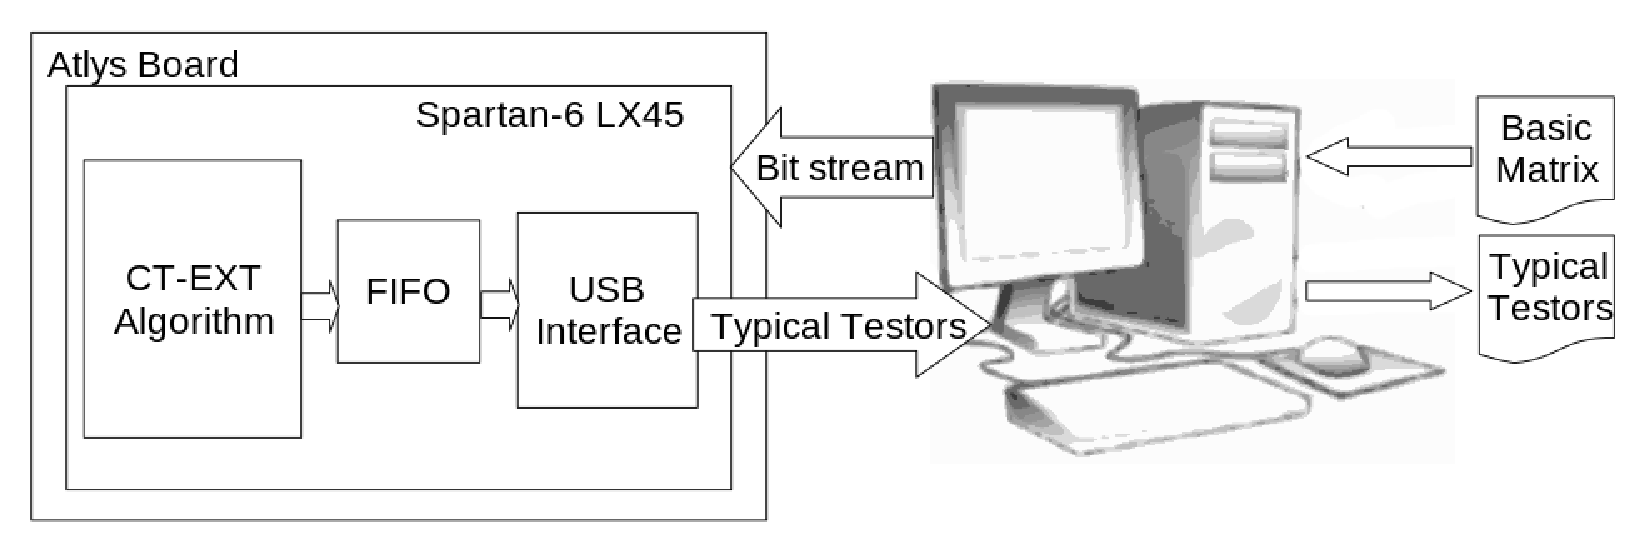
\includegraphics[width=13cm]{Arquitecture.eps}
    \end{center}
\caption{Proposed hardware-software platform.}
\label{figArq}
\end{figure}

\section{Hardware architecture}
\label{sect:4}

\begin{figure}[htb]
    \begin{center}
        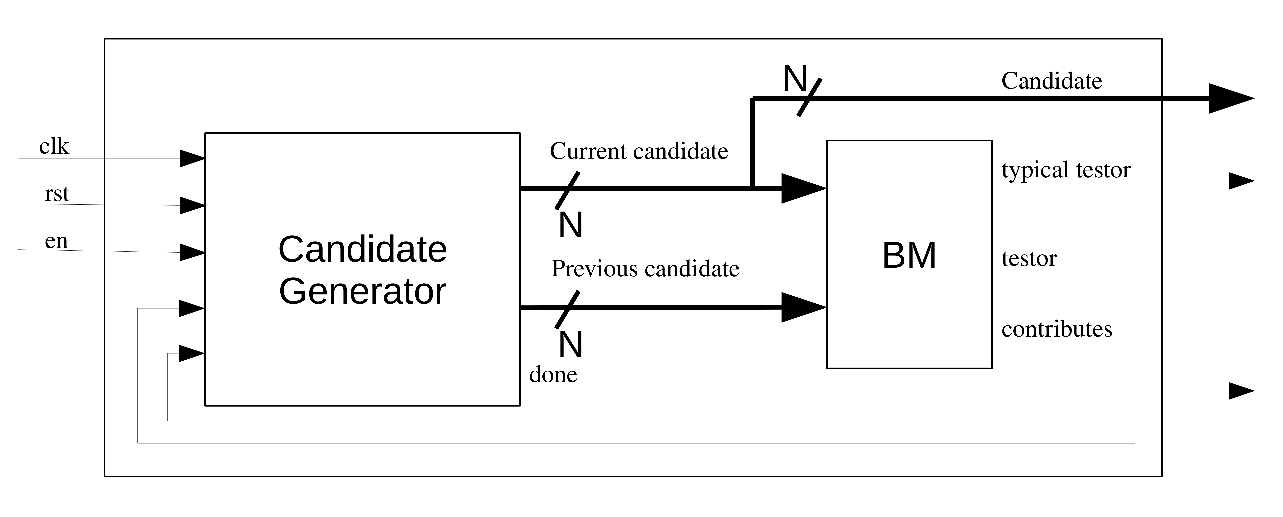
\includegraphics[width=13cm]{CT-ext_arq.eps}
    \end{center}
\caption{CT-EXT Architecture.}
\label{fig:3}
\end{figure}

The process of deciding whether an $N$-tuple is a testor of $BM$ involves
comparing the candidate against each one of the $BM$'s rows. For
software-only implementations, this is a big disadvantage, in
particular for large matrices with many rows. The proposed hardware
architecture exploits the parallelism inherent in the CT-EXT algorithm
and evaluates whether a candidate is an irreducible testor or not in a single
clock cycle. It is composed by two main modules as seen in
Fig.\,\ref{fig:3}. 

The $BM$ module stores the input matrix and
includes logic to decide whether an $N$-tuple is a testor. The candidate
generator module produces the candidates ($N$-tuples) to be
evaluated by the $BM$ module. In order to calculate the next candidate
according to the CT-EXT algorithm, the architecture feedbacks the
evaluation result of the previous candidate to the generator module,
this allows to drastically reduce the number of candidates tested
thus the number of iterations needed by the algorithm. At this
point, the architecture is able to obtain all testors of $BM$,
however since only irreducible testors are of interest, a final
hardware processing module eliminates most of the testors that are
not irreducible before sending the remaining testors to the software
for final processing. The dismiss module exploits the way
consecutive testors are obtained. If a testor is a superset of at
least one previous testor, it is not an irreducible testor, thus it
is eliminated. This final process does not introduce delays, thus
the architecture is still capable of evaluating a candidate in a
single clock cycle.

\begin{figure}[htb]
    \begin{center}
        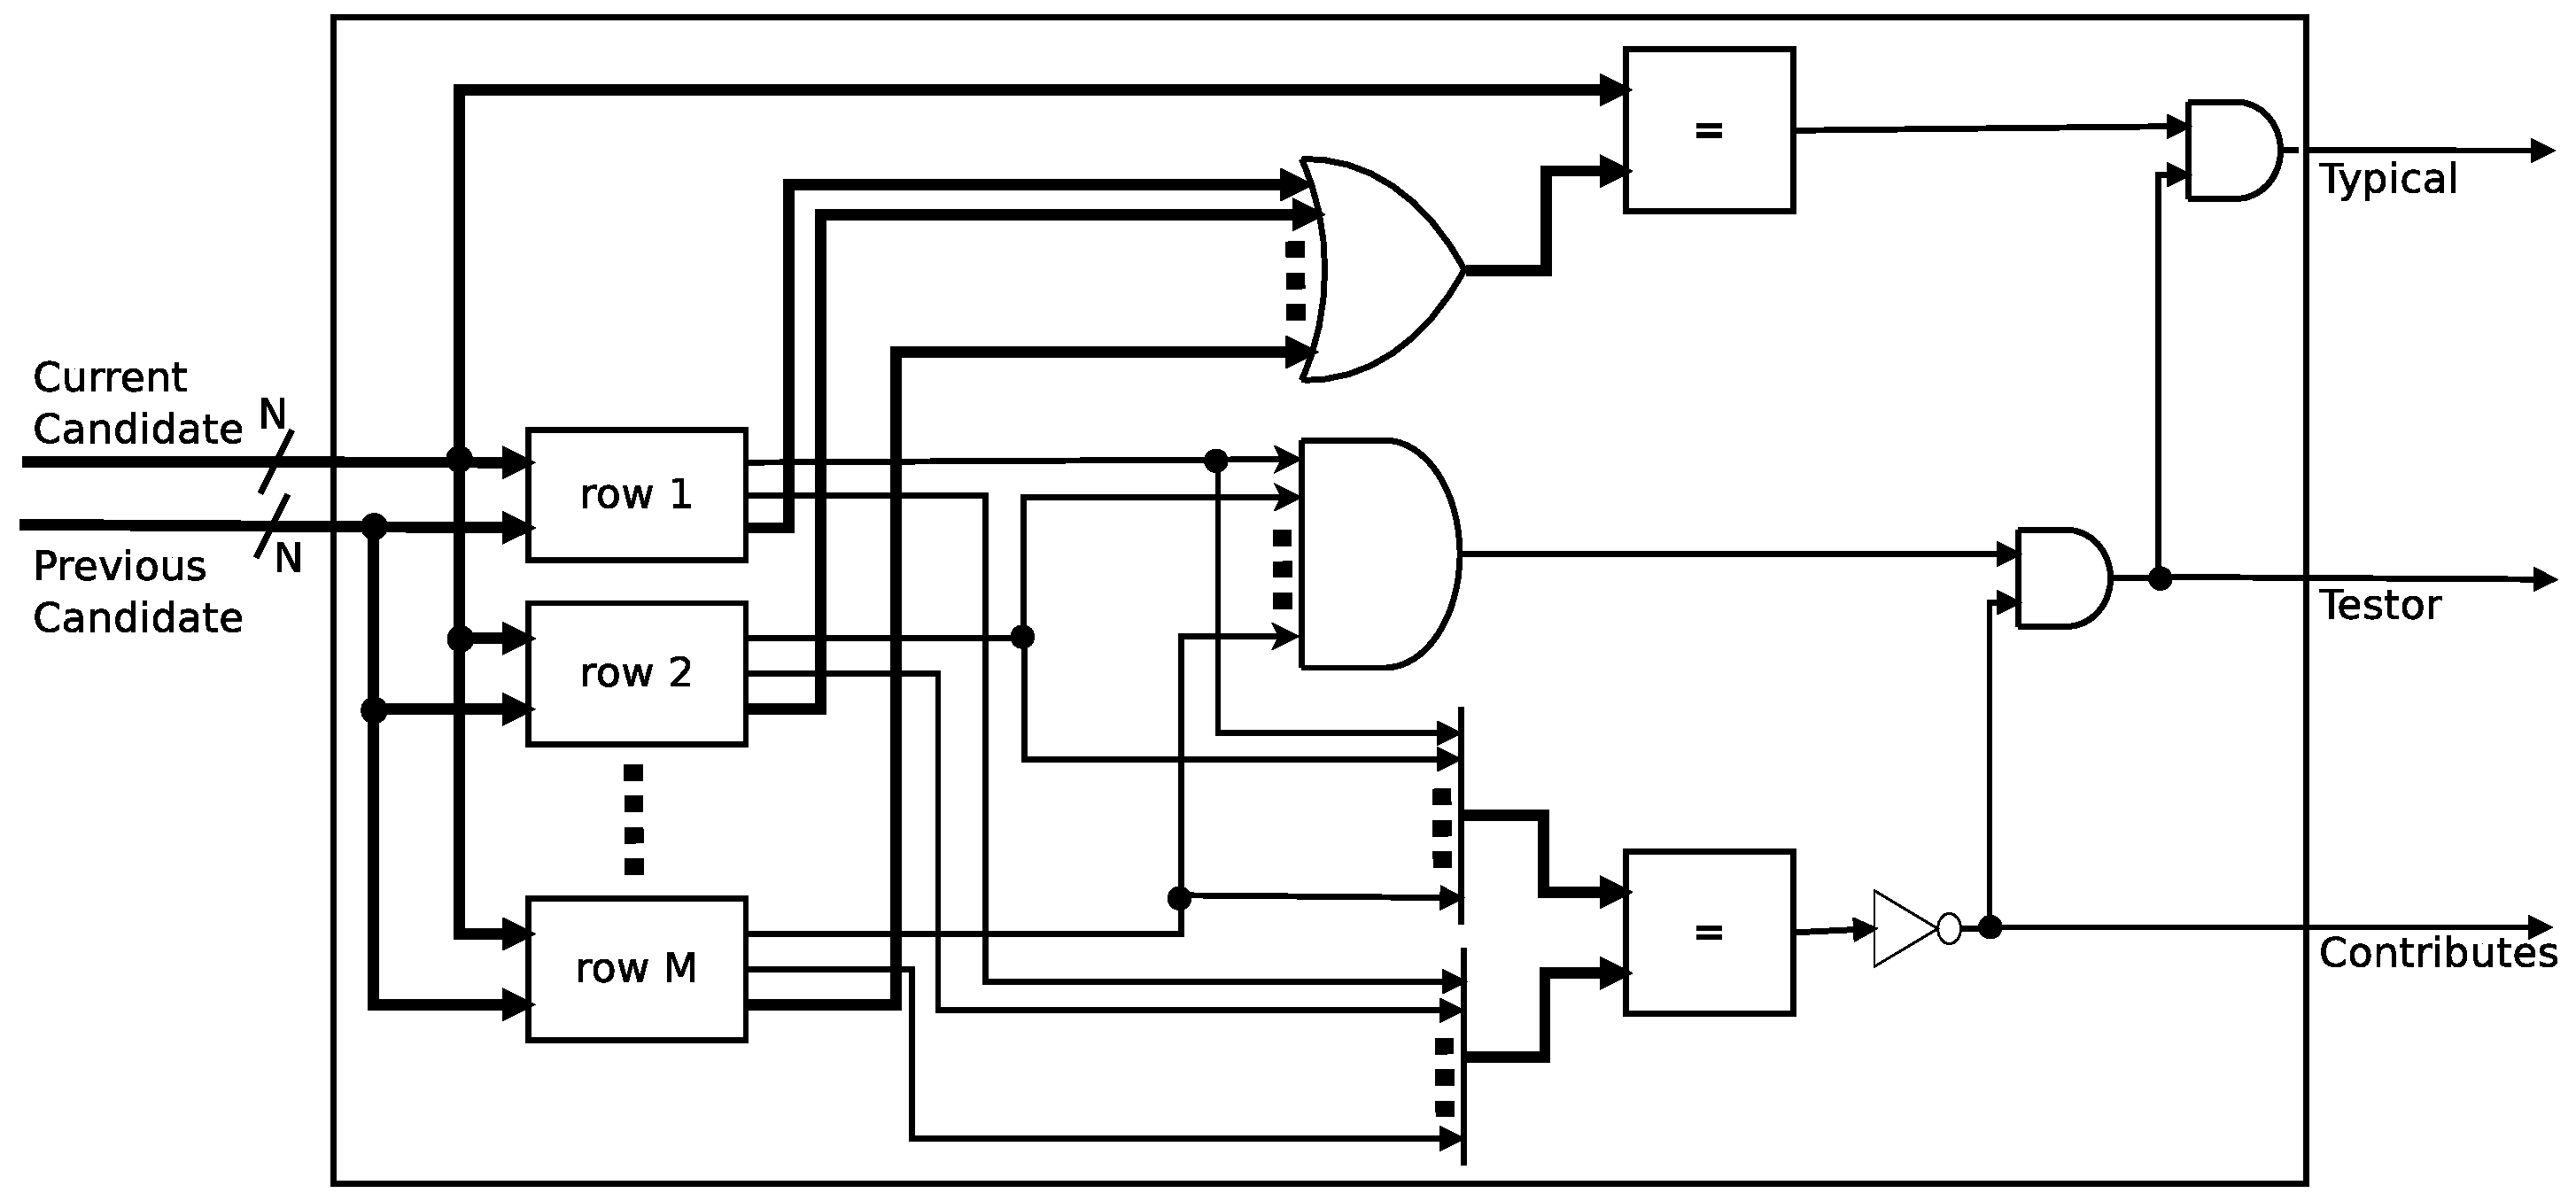
\includegraphics[height=6cm]{BM_module.eps}
    \end{center}
\caption{$BM$ module.}
\label{fig:4}
\end{figure}

The $BM$ module is composed of $M$ sub-modules named \textit{row~x}, as shown
in Fig.\,\ref{fig:4}. Each \textit{row~x} module contains a row ($N$ bits)
of the $BM$ matrix and logic to perform testor evaluation. To decide
if an $N$-tuple is a testor, a bitwise AND operation is performed
between the constant stored in each \textit{row~x} module and the current
candidate as shown in Fig.\,\ref{fig:row}. If at least one bit of the AND operation result is TRUE,
then the output \textit{Testor} of that particular \textit{row~x} sub-module
will be TRUE. The same operation is performed over the previous candidate.
If the count of rows asserting the output \textit{Testor} is different from
those asserting the output \textit{Contributes} of that particular \textit{row~x} sub-module, 
then output \textit{Contributes} from the $BM$ module becomes TRUE.
If the outputs of all  \textit{row~x} sub-modules are
TRUE, then the output \textit{Testor} of the $BM$ module will be TRUE,
which means that the candidate is declared a testor of $BM$.

\begin{figure}[htb]
    \begin{center}
        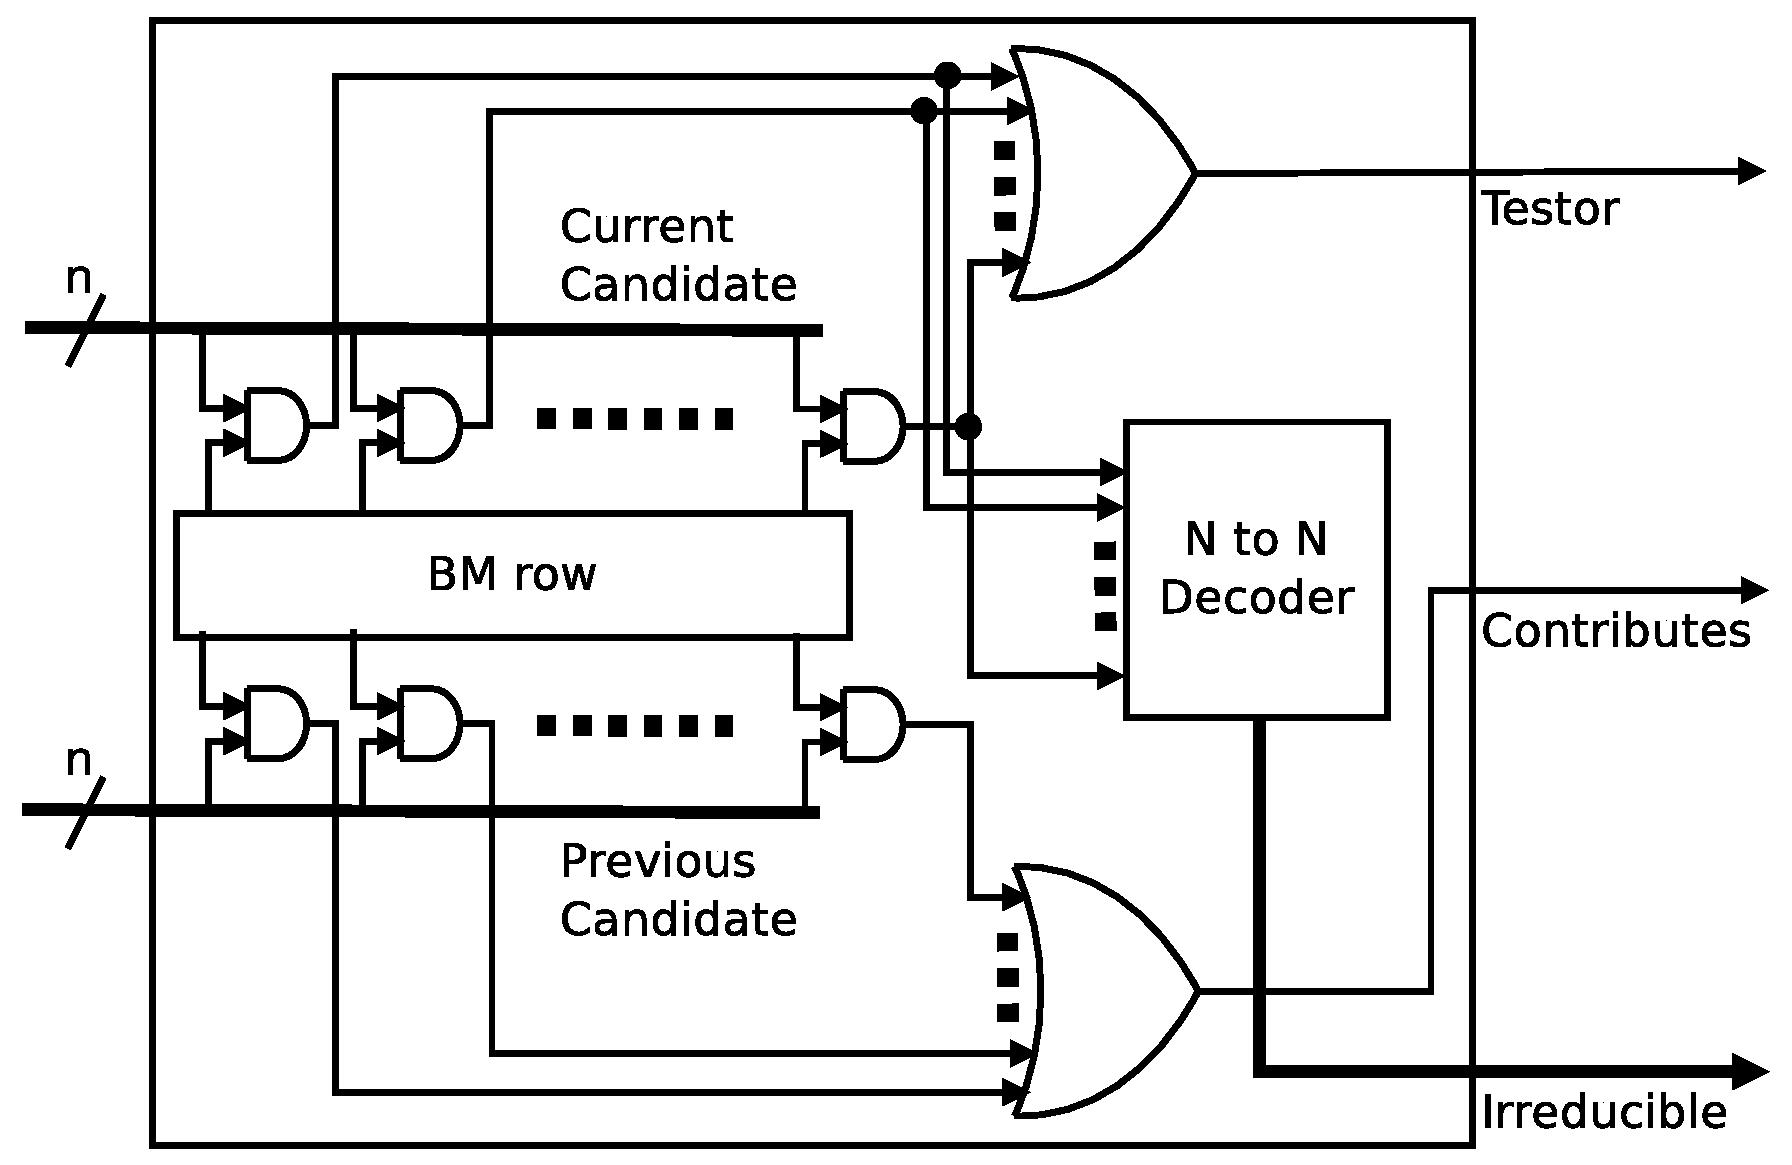
\includegraphics[height=6cm]{BM_row.eps}
    \end{center}
\caption{$BM$ row.}
\label{fig:row}
\end{figure}

In order to check the irreducible condition of testors, the module \textit{N to N decoder}
receives as input the result of AND operation between the current candidate and the $BM$ row.
The output from module \textit{N to N decoder} repeats the input in case there is only one bit set
in it, and returns zero otherwise. For those rows with only one bit set after anded with candidate,
the attribute in the position of setted bit is indispensable in case the candidate be a testor.
According to definition~\ref{def24}, every attribute in a testor must be indispensable to be an
irreducible testor. %This idea is stated in definition~1 of \citep{R13}.

\setlength{\tabcolsep}{3pt}
\begin{table}[!htb]
    \begin{minipage}{.5\linewidth}
      \caption{Irreducible testor.}\label{table4}
      \centering
        \begin{tabular}{ ccccc|ccccc }
 			\hline                       
  			\multicolumn{5}{c|}{Cand. $(x_0 x_1)$} & 
  			\multicolumn{5}{c}{Decoder output} \\
  			\hline
  			%\multicolumn{5}{c|}{$x_0~x_3~x_4~x_1~x_2$}&\multicolumn{5}{c}{$x_0~x_3~x_4~x_1~x_2$}\\
  			$x_0$ & $x_3$ & $x_4$ & $x_1$ & $x_2$ &
  			$x_0$ & $x_3$ & $x_4$ & $x_1$ & $x_2$ \\
  			\hline
  			1 & 0 & 0 & 0 & 0 & 1 & 0 & 0 & 0 & 0\\
  			0 & 0 & 0 & 1 & 0 & 0 & 0 & 0 & 1 & 0\\
  			1 & 0 & 0 & 1 & 0 & 0 & 0 & 0 & 0 & 0\\
  			\hline  
  			\multicolumn{5}{c|}{Candidate $=$} & 1 & 0 & 0 & 1 & 0\\
  			\hline  
		\end{tabular}
	%\end{table}
	%\begin{table}[!htb]
    \end{minipage}%
    \begin{minipage}{.5\linewidth}
      \centering
        \caption{Is not an irreducible testor.}\label{table5}
        \begin{tabular}{ ccccc|ccccc }
 			\hline                       
  			\multicolumn{5}{c|}{Cand. $(x_0 x_4)$} & 
  			\multicolumn{5}{c}{Decoder output} \\
  			\hline
  			%\multicolumn{5}{c|}{$x_0~x_3~x_4~x_1~x_2$}&\multicolumn{5}{c}{$x_0~x_3~x_4~x_1~x_2$}\\
  			$x_0$ & $x_3$ & $x_4$ & $x_1$ & $x_2$ &
  			$x_0$ & $x_3$ & $x_4$ & $x_1$ & $x_2$ \\
  			\hline
  			1 & 0 & 1 & 0 & 0 & 0 & 0 & 0 & 0 & 0\\
  			0 & 0 & 1 & 0 & 0 & 0 & 0 & 1 & 0 & 0\\
  			1 & 0 & 1 & 0 & 0 & 0 & 0 & 0 & 0 & 0\\
  			\hline  
  			\multicolumn{5}{c|}{Candidate $\neq$} & 0 & 0 & 1 & 0 & 0\\
  			\hline  
		\end{tabular}
    \end{minipage} 
\end{table}

Taking as  example the ordered basic matrix in table~\ref{table2}. In table~\ref{table4} the irreducibility of candidate $\{x_0,x_1\}$ is evaluated while the same is done for candidate $\{x_0,x_4\}$ in table~\ref{table5}. Left rows show the result of the AND operation between each row of $BM$ and the candidate, while those rows in the right show decoder output taking as input the cell in its left. In the last row the result of OR operation over all cells above is shown. According to our previous explanation, candidate $\{x_0,x_1\}$ is an irreducible testor been equal to the OR operation result while candidate $\{x_0,x_4\}$ is not. This can be corroborated in table~\ref{tab_example}.

\begin{figure}[t]
    \begin{center}
        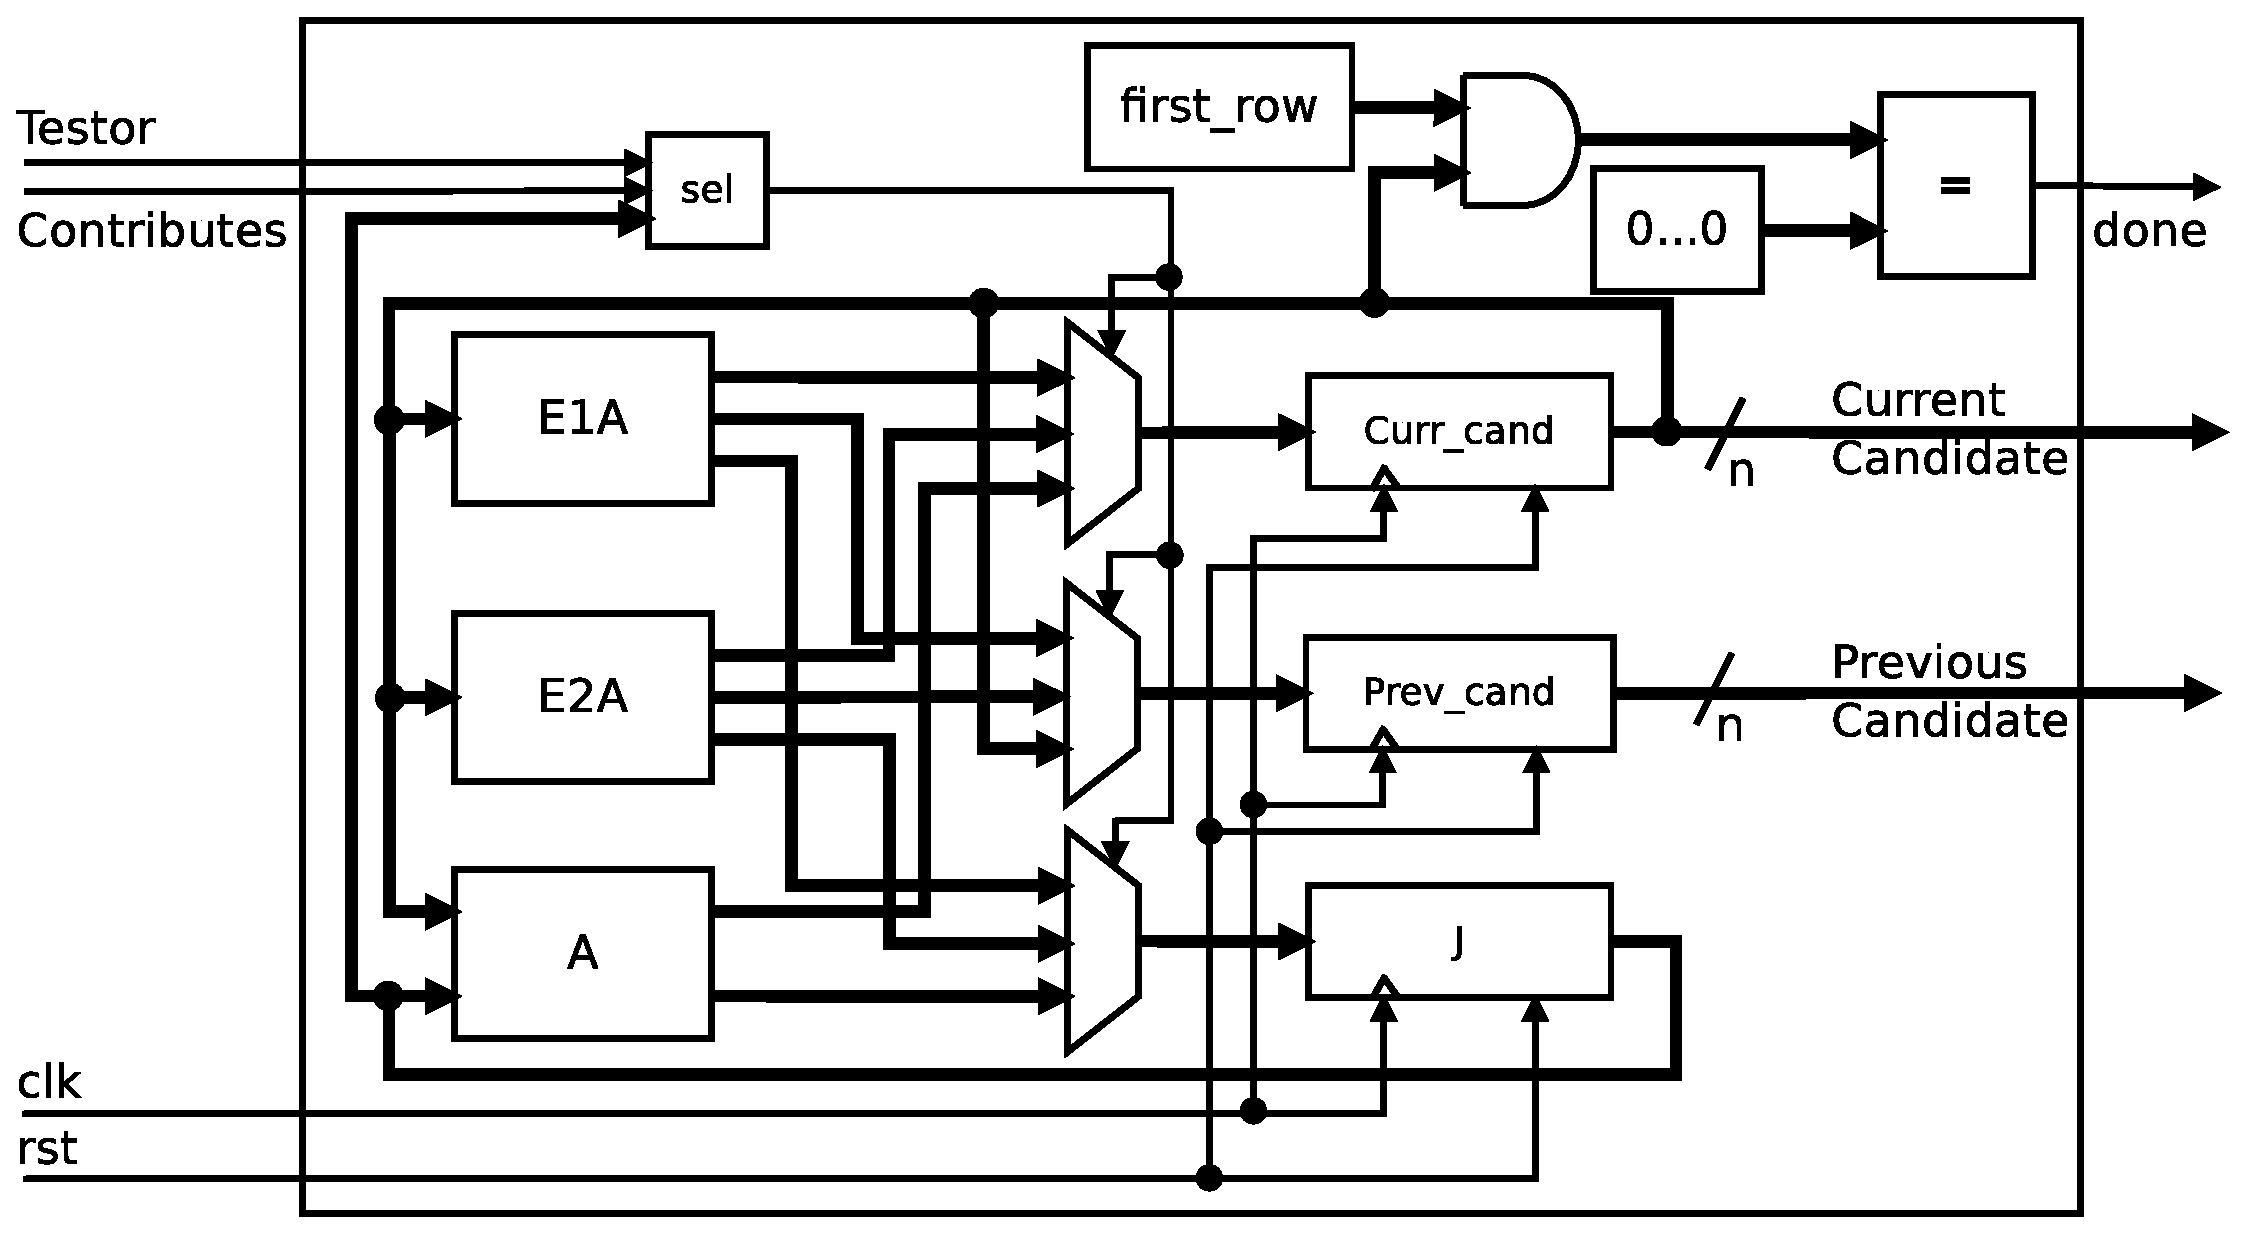
\includegraphics[height=6cm]{CandGen.eps}
    \end{center}
\caption{Candidate Generator module.}
\label{fig:5}
\end{figure}

The candidate generator module uses the feedback from the $BM$ module
to calculate the next candidate to be evaluated. The
candidate generator module (Fig.\,\ref{fig:5}) consists of three
registers for holding the current candidate (\textit{Curr$\_$cand}), the previous candidate
(\textit{Prev$\_$cand}) and the last added attribute ($J$). These registers values are updated
by the modules EA1, EA2 and A.

Depending on the combination of input values, the outputs E1A,
E2A or A are taken to update the records accordingly. Table~\ref{tab_CandGen} shows the
conditions that must be met by \textit{Testor}, \textit{Contributes} and $J$ inputs, such that each
register receives the correct value and the priority that should be evaluated. This
operation is computed in module \textit{sel} from figure~\ref{fig:5}.

 \begin{table}[htb]
		\caption{Candidate Generator Selector.} \label{tab_CandGen}
		\centering
 	\begin{tabular}{ccc}
 			\hline
 			Priority & Condition & Registers update\\
 			\hline
 			1 & \multicolumn{1}{>{\centering\arraybackslash}m{1in}}{$J=J_{max}$
 				($J_{max}=$ max value of $J$)} & \multicolumn{1}{>{\centering\arraybackslash}m{2in}}{
 				curr$\_$cand $\leftarrow$ E2A
 				prev$\_$cand~$\leftarrow$~E2A
 				$J$~$\leftarrow$~E2A}\\
 			\hline
 			2 & \multicolumn{1}{>{\centering\arraybackslash}m{1.2in}}{Contributes $=0$ or Testor $=1$} &
 			\multicolumn{1}{>{\centering\arraybackslash}m{2in}}{
 				curr$\_$cand $\leftarrow$ E1A
 				prev$\_$cand~$\leftarrow$~E1A
 				$J$~$\leftarrow$~E1A}\\
 			\hline
 			3 & \multicolumn{1}{>{\centering\arraybackslash}m{1.2in}}{Contributes $=1$ or Testor $=0$}&
 			\multicolumn{1}{>{\centering\arraybackslash}m{2in}}{
 				curr$\_$cand $\leftarrow$ A
 				prev$\_$cand~$\leftarrow$~curr$\_$cand
 				$J$~$\leftarrow$~A}\\
 			\hline       
 	\end{tabular}             
 \end{table}

The submodule $A$ from Fig.\,\ref{fig:subA} sets the attribute following the last bit setted in
the input candidate. Its outputs are the new candidate and the incremented by one $J$ value.

The submodule $E1A$  from Fig.\,\ref{fig:subEA1} comprises the \textit{Rem$\_1$} 
(Fig.\,\ref{fig:subRem1}) and $A$ submodules. 
The submodule \textit{Rem$\_1$} deletes the last attribute added to the input candidate. 
This action is performed by a priority encoder which locates the last bit setted in the input candidate. 
\textit{Rem$\_1$} outputs represent the index of cleared bit. 
%: $J$ and \textit{candidate} which is the input candidate without the last attribute. 
These outputs are connected to the corresponding inputs of 
submodule $A$ in order to add an attribute in the corresponding position. Finally, the outputs of $E1A$ are 
the new candidate to be evaluated, and the index where the new attribute is added to the 
candidate, both outputs of $A$.


\begin{figure}[htb]
\centering
\begin{minipage}{.5\textwidth}
  \centering
   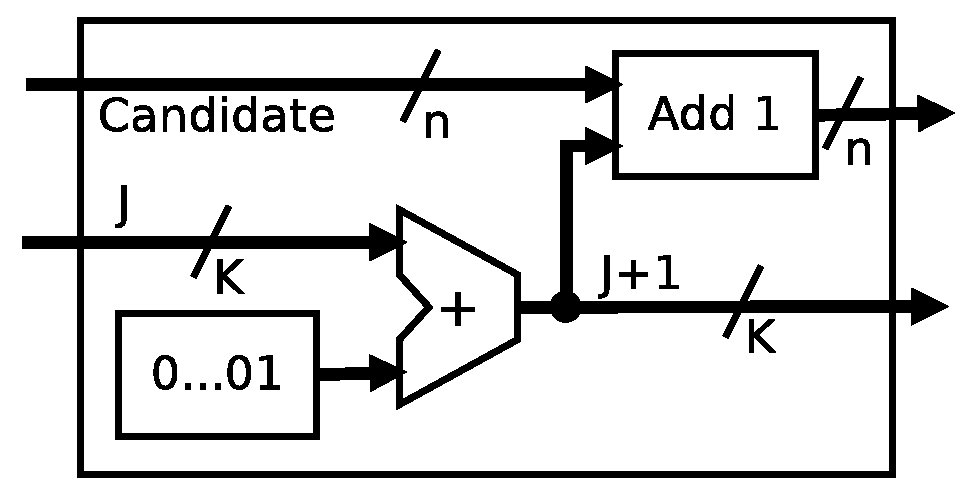
\includegraphics[width=.7\linewidth , height=3cm]{Add1.eps}
  \caption{Submodule A.}
  \label{fig:subA}
\end{minipage}%
\begin{minipage}{.5\textwidth}
  \centering
   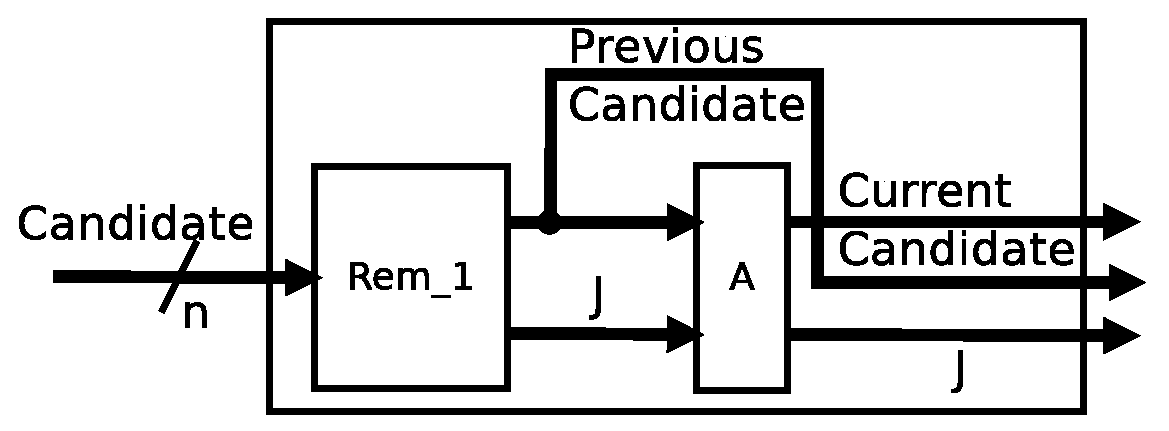
\includegraphics[width=\linewidth , height=3cm]{EA1.eps}
  \caption{Submodule E1A.}
  \label{fig:subEA1}
\end{minipage}
\end{figure}

Finally, submodule $E2A$ is responsible for removing the last two attributes from
input candidate, and then adding the following corresponding attribute. This 
operation is performed by means of two \textit{Rem$\_1$} submodules and a submodule $A$, as 
shown in Fig.\,\ref{fig:subEA2}.

In order to check the termination  of the algorithm the result of AND operation between current candidate and
the first row of the basic matrix is compared to the null $N$-tuple ($0,...,0$), as shown in 
upper right corner of Fig.\,\ref{fig:5}. In case of TRUE comparison the output done is activated 
because any other combination in the order will not satisfy the condition over the first row of $BM$.

\begin{figure}[htb]
\centering
\begin{minipage}{.5\textwidth}
  \centering
   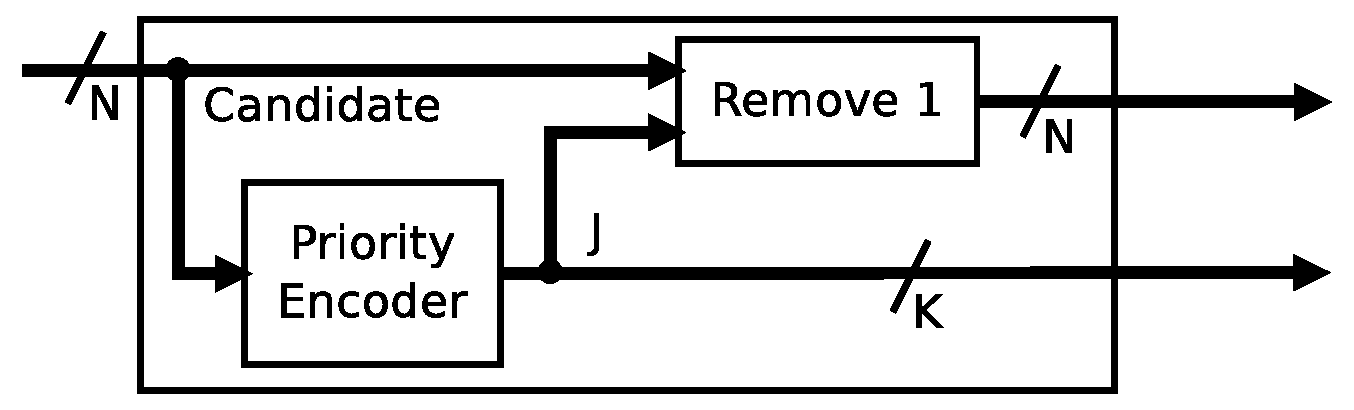
\includegraphics[width=\linewidth , height=3cm]{Rem1.eps}
  \caption{Submodule Rem$\_1$.}
  \label{fig:subRem1}
\end{minipage}%
\begin{minipage}{.5\textwidth}
  \centering
   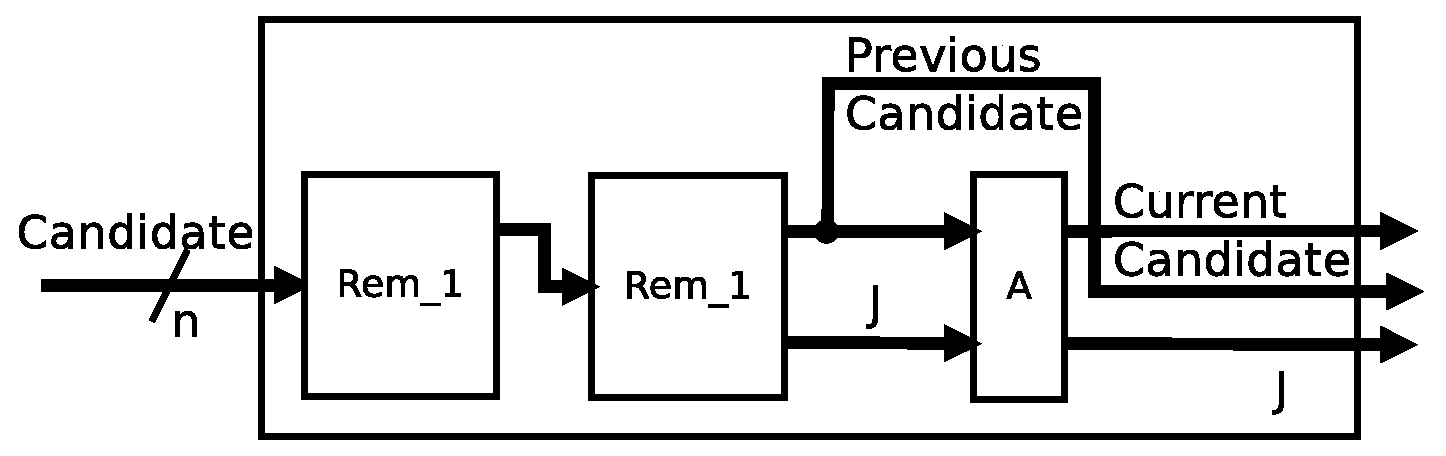
\includegraphics[width=\linewidth , height=3cm]{EA2.eps}
  \caption{Submodule E2A.}
  \label{fig:subEA2}
\end{minipage}
\end{figure}

The prototyping board used \citep{R15} allows the communication between the PC and the FPGA 
through USB port. Irreducible testors are buffered into a FIFO in order to be split into
bytes which are then buffered into a double clocked FIFO \citep{R26} to be read from the PC using 
DSTM  \citep{R25} protocol.

\section{Software Description}
\label{sect:5}

The software component consists of a command line interface. The user must provide the basic matrix in a 
plain text file in the format shown in Fig.\,\ref{fig:8}. This software is responsible for programming the 
FPGA device and communicating with the board during operation.

%The software component works as an
%interface between the user, the computer, and the FPGA board. The
%input data file must be in plain text following the format shown in
%Fig.\,\ref{fig:8}.

On command line program call, the basic matrix is read from the input file. Once the
data is loaded into memory, the basic matrix is reorganized by setting the row with 
minimum amount of ones as the first row and swapping columns in such a way the ones in 
first row appear on the left, no matters the order between them.
Then, in order to complete the project files, one VHDL file
is generated and synthesis process is started, producing the programming file for the FPGA
device.

On running stage, software component interact with hardware architecture. 
First, the device is programmed with the bit-file obtained from the previous stage,
given that the board is powered and properly connected to the hosting PC. Now, the
hardware architecture starts computing irreducible testors. 
Software keeps pulling through USB for new irreducible testors in the output 
FIFO until done is activated in the FPGA.

Finally irreducible testors are codified according to the original order of
columns and written to output file.

\begin{figure}[t]
    \begin{center}
        \includegraphics[height=2.8cm]{infile.eps}
    \end{center}
\caption{Input file format.}
\label{fig:8}
\end{figure}

\section{Evaluation}
\label{sect:6}

%\begin{table*}[t]%[tpb]
%    \caption{Processing time in seconds (broken down for each stage) for 45X100 low, medium and high density matrices.}
%    \label{table:5}
%    \begin{center}
%        %\scalebox{.7}{
%        \begin{tabular}{ccccccc} \cline{2-7}
%             & \multicolumn{2}{c}{\bf Low Density} & \multicolumn{2}{c}{\bf Medium Density} & \multicolumn{2}{c}{\bf High Density} \\ \hline
%            Stages & HW/SW & SW-O & HW/SW & SW-O & HW/SW & SW-O \\ \hline
%            Load BM & 0.031 & 0.031 & 0.031 & 0.031 & 0.032 & 0.031 \\
%            BM arrangement & 0.281 & 0.281 & 0.281 & 0.024 & 0.282 & 0.01 \\
%            Files creation & 0.032 & N/A \footnote[1]{Not Applicable} & 0.031 & N/A\footnote[1]{Not Applicable} & 0.046 & N/A\footnote[1]{Not Applicable} \\
%            Synthesis & 691 & N/A\footnote[1]{Not Applicable} & 1,032 & N/A\footnote[1]{Not Applicable} & 930 & N/A\footnote[1]{Not Applicable} \\
%            IT\footnote[2]{Irreducible testors.} computing & 316 & 170,830 & 1,303 & 51,777 & 8 & 0.06 \\ \hline
%            TOTAL & 1,008 & 170,831 & 2,336 & 51,778 & 939 & 0.11 \\ \hline
%        \end{tabular}%}
%    \end{center}
%\end{table*}

%- 2 dif dens y 1 real
%- dependence on BM
%- sintesis overhead


In order to show the performance of the proposed platform, it was compared against a software 
implementation of the CT-EXT algorithm and BT hardware platform from \citep{R21}. 
For experimentation purposes, BT hardware platform was modified for finding irreducible testors 
on the FPGA as we explained in section~\ref{sect:4}.

In order to understand experiments design, some ideas on algorithms and implementations must be commented. 
Either CT-EXT or BT (modified) hardware implementations are capable of evaluating a candidate per clock 
cycle. If both architectures are running at the same frequency, as will be the case in our experiments, 
there are two reasons for differences in running time. The first one is the time taken to matrix 
reorganization, which is a more complex process for BT, but it can be neglected as shown in \citep{R21}. 
The second and relevant one, is the amount of candidates to be evaluated. It is not a difficult task 
to find a $BM$ in which BT evaluates less candidates than CT-EXT or vice versa.

In relation to software implementation, the CT-EXT hardware platform has two disadvantages. First, 
VHDL code is generated with $BM$ data and a process of synthesis is executed previous to algorithm 
execution while this is unnecessary in software platform. Secondly, the software will be running in 
a PC at a frequency of 3.10GHz while FPGA architecture will be at 50MHz. 

These disadvantages make the hardware approach useful (faster) under two conditions. The algorithm 
execution must require the evaluation of a number of candidates big enough to overcome the synthesis 
overhead; and the dimensions of the $BM$ must be big enough to provide a gain in a single candidate 
evaluation. Although hardware architecture could be design for a fixed maximum matrix size and 
receive the $BM$ through USB, the size of the problem would be significantly reduced. The synthesis 
process comprehend an optimization of the design, taking advantage of $BM$ data for the reduction of 
generated hardware. The number of operations for the evaluation of a single candidate in the software 
approach is proportional to the number of rows and has a relation with the number of columns in the 
$BM$. CPU operations will be increased every time the number of attributes exceeds a multiple of 
microprocessor word width. This way we can have a gain, even at a much lower running frequency, from 
evaluating a candidate every clock cycle.

With these restrictions in mind, to show the usability of proposed platform, 
two kinds of basic matrices were randomly generated. Each type containing different amount of 1's per 
row and different amount of rows. Here after we will be discerning between these two series of matrices 
by its density of 1's.
Additionally, a basic matrix obtained from real data (\textbf{CITE}) is used.
%Intel(R) Core(TM) i5-2400 CPU @ 3.10GHz
Several basic matrices of different sizes were randomly generated for each kind. On hardware platforms 
the runtimes for the following stages: $BM$ input parsing and VHDL code generation, synthesis of ISE project, 
and irreducible testor computation (with a hardware frequency of 50MHz), were measured. 
Figs.\,\ref{fig:result1}, and \,\ref{fig:result2} show graphs of the whole processing time for the two kind 
of basic matrices. 

\begin{figure}[htb]
\centering
\begin{minipage}{.5\textwidth}
  \centering
   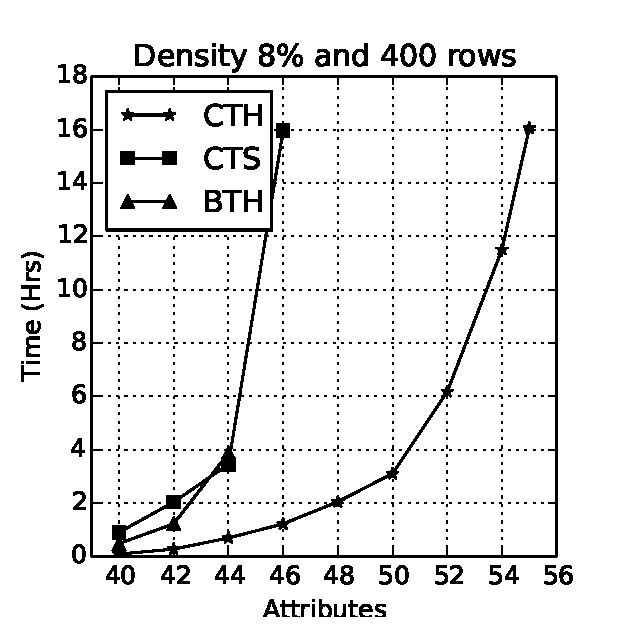
\includegraphics[width=\linewidth , height=5.5cm]{low_density.eps}
  \caption{Total runtime for density 8\%.}
  \label{fig:result1}
\end{minipage}%
\begin{minipage}{.5\textwidth}
  \centering
   \includegraphics[width=\linewidth , height=5.5cm]{med_density.eps}
  \caption{Total runtime for density 30\%.}
  \label{fig:result2}
\end{minipage}
\end{figure}

Tables~\ref{sect:6} and~\ref{table:7} summarize the FPGA resources utilization on our prototyping board. 
As we can see, CT-EXT implementation is smaller than modified BT implementation. Resources utilization is 
related to $BM$ dimensions and density and to a lesser extent to data organization.

\begin{table}[htb]
\caption{Synthesis summary of resources utilization for $BM$ with 8\% density on Spartan-6 LX45 
FPGA device.} \label{table:6}
\begin{center}
    \begin{tabular}{lcccc}   \hline
    	    Dimensions & \multicolumn{2}{c}{400x40} & \multicolumn{2}{c}{400x44} \\ \hline
    	    Algorithm & BT & CT-EXT & BT & CT-EXT \\ \hline
        Slices & 1,398 (20\%) & 983 (14\%) & 1,554 (22\%) & 1,209 (17\%)  \\
        6-input LUTs & 4,010 (14\%) & 2,806 (10\%)& 4,475 (16\%)  & 3,004 (11\%)\\
        Flip-Flops & 832 (1\%) & 852 (1\%) & 876 (1\%) & 938 (1\%)\\
        Max clock freq & 80.44MHz & 179.58MHz & 84.56MHz & 173.24MHz\\ \hline
    \end{tabular}
\end{center}
\end{table}

\begin{table}[htb]
\caption{Synthesis summary of resources utilization for $BM$ with 30\% density on Spartan-6 LX45 
FPGA device.} \label{table:7}
\begin{center}
    \begin{tabular}{lcccc}   \hline
    	    Dimensions & \multicolumn{2}{c}{225x50} & \multicolumn{2}{c}{225x55} \\ \hline
    	    Algorithm & BT & CT-EXT & BT & CT-EXT \\ \hline 
        Slices & 1,381 (20\%) & 1,554 (22\%) & 1,455 (21\%) & 1,562 (22\%) \\
        6-input LUTs & 3,769 (13\%) & 4,315 (15\%) & 4,135 (15\%) & 5,026 (18\%)\\
        Flip-Flops & 949 (1\%) & 980 (1\%) & 1,002 (1\%) & 1,039 (1\%)\\
        Max clock freq & 87.46MHz & 155.40MHz & 85.27MHz & 156.35MHz\\ \hline
    \end{tabular}
\end{center}
\end{table}

%\begin{table*}[t]%[tpb]
%\caption{FPGA Resource utilization for Virtex II XC2V3000 for $N=50$ and $M=100$ (Whole
%architecture vs Dismis testors module).}
% \label{table:7}
%\begin{center}
%    %\scalebox{.68}{
%    \begin{tabular}{ccccccc} \cline{2-7}
%         & \multicolumn{2}{c}{\bf8 REG\_DT} & \multicolumn{2}{c}{\bf16 REG\_DT} & \multicolumn{2}{c}{\bf32 REG\_DT} \\ \hline
%         & Whole & Dismiss & Whole & Dismiss & Whole & Dismiss \\
%        \raisebox{1.5ex}[0pt]{\bf Resources} & architecture & Testors & architecture & Testors & architecture & Testors \\ \hline
%        Slices & 2365 & 338 & 2676 & 679 & 3331 & 1342 \\
%        Flip-flops & 1024 & 400 & 1451 & 800 & 2236 & 1600 \\
%        LUTs & 4256 & 258 & 4472 & 472 & 4871 & 892 \\ \hline
%    \end{tabular}%}
%\end{center}
%\end{table*}

%where $f$ is the clock frequency of the architecture and $c$ is the
%percentage of candidates tested. Note that the value of $c$ is data
%dependent, i.e. it varies for each basic matrix, $BM$.
%
%It is important to notice that the processing time for computing
%irreducible testors does not only depend on the size and density of
%the $BM$, but also on the distribution of 0's and 1's inside the
%matrix. This assertion can be appreciated in points 43 to 45 of
%Fig\,\ref{fig:11}.

%Table\,\ref{table:5} shows the processing time for each stage of the data flow, for 45X100 low, medium, and
%high density matrices. This table shows that the proposed platform allows running BT 169 times faster that
%the software-only implementation, for a 45X100 low density matrix and 22 times faster for the medium density
%matrix of the same size. Moreover, taking into account only the last stage of the data flow, the improvement
%over the software is 540X for the low density matrix and 39X for the medium density one. The only type of
%matrices where the proposed platform does not perform better that the software-only BT implementation was the
%high density ones, this is because of computing irreducible testors is very fast for this kind of matrices.
%The software-only implementation of BT was executed on a PC with an Intel Centrino Duo processor running at
%1.6GHz, with 1024 MB of RAM.

%The proposed platform has been designed to process variable sizes of the $BM$ matrix. The maximum size of the
%matrix that can be implemented is only limited by the available resources on the specific FPGA board. For
%example, for the Virtex-II XC2V3000 from Xilinx\cite{R14} embedded on an XtremeDSP board \citep{R15}, the
%biggest medium density matrix that can fit into the FPGA is about 100X325. Table\,\ref{table:6} summarizes
%the resource utilization for this matrix.
%
%Finally, Table\,\ref{table:7} summarizes the resource utilization
%for a 50X100 matrix for different buffer sizes on the Dismiss Testor
%module, all for the same device. Although 8 and 32 are good choices,
%16 results in a better trade-off between resource utilization (small
%when compared against the whole architecture), and the non
%irreducible testors eliminated (always over 79\%, as
%Table\,\ref{table:4} shows).

\section{Discussion}
\label{sect:7}

The proposed hardware platform provides higher processing
performance than the software implementation of the CT-EXT
algorithm for matrices used in the experimentation. 
This behaviour is possible because the hardware
component of the proposed platform is capable of testing if a 
candidate is a testor of a $BM$ in a single clock cycle,
independently of the number of columns and rows, whereas
software implementation processing time will significantly
increase for matrices with a large number of rows.

Moreover, the performance improvement is directly related to the
percentage of candidates tested ($c$), which heavily depends on
density and distribution of the values into the $BM$ matrix. This occurs in the
software as well as in the hardware implementation,
but the proposed platform also needs to synthesize the specific
architecture. For practical purposes, a concurrent approach can be used 
in computation of irreducible testors. This way, the same $BM$ is provided 
to hardware and software implementations of BT and CT-EXT algorithms at the same time. 
We can get the answer from the faster one without knowing which will be the best 
for the given data.

Experiment results show that the proposed platform beats the software implementation of
the CT-EXT algorithm, with rates of \textbf{one order} of magnitude. However, for large 
enough data set this improvement could be significantly higher.

\section{Conclusions}
\label{sect:8}

The high performance of hardware implementation is feasible due to the
high level of parallelism implicit in candidates evaluation of algorithms which can be
efficiently implemented on an FPGA. 
Proposed platform improves our previous architecture \citep{R21} by finding \textit{irreducible} testors 
in a single clock cycle. This new feature solves problems arising from transmission of irrelevant 
data to the hosting PC while improves total execution time. 

Main drawback of proposed platform is the limitation in matrix dimensions depending on FPGA 
device capacity. Reducing the clock frequency allows the implementation of larger matrices at the 
cost of slower execution.

Proposed architecture offers an alternative to BT algorithm which will be faster in must cases. 
Improvements, such as testing two or more candidates per iteration,
are still unexplored.


%% The Appendices part is started with the command \appendix;
%% appendix sections are then done as normal sections
%% \appendix

%% \section{}
%% \label{}

%% References
%%
%% Following citation commands can be used in the body text:
%%
%%  \citet{key}  ==>>  Jones et al. (1990)
%%  \citep{key}  ==>>  (Jones et al., 1990)
%%
%% Multiple citations as normal:
%% \citep{key1,key2}         ==>> (Jones et al., 1990; Smith, 1989)
%%                            or  (Jones et al., 1990, 1991)
%%                            or  (Jones et al., 1990a,b)
%% \cite{key} is the equivalent of \citet{key} in author-year mode
%%
%% Full author lists may be forced with \citet* or \citep*, e.g.
%%   \citep*{key}            ==>> (Jones, Baker, and Williams, 1990)
%%
%% Optional notes as:
%%   \citep[chap. 2]{key}    ==>> (Jones et al., 1990, chap. 2)
%%   \citep[e.g.,][]{key}    ==>> (e.g., Jones et al., 1990)
%%   \citep[see][pg. 34]{key}==>> (see Jones et al., 1990, pg. 34)
%%  (Note: in standard LaTeX, only one note is allowed, after the ref.
%%   Here, one note is like the standard, two make pre- and post-notes.)
%%
%%   \citealt{key}          ==>> Jones et al. 1990
%%   \citealt*{key}         ==>> Jones, Baker, and Williams 1990
%%   \citealp{key}          ==>> Jones et al., 1990
%%   \citealp*{key}         ==>> Jones, Baker, and Williams, 1990
%%
%% Additional citation possibilities
%%   \citeauthor{key}       ==>> Jones et al.
%%   \citeauthor*{key}      ==>> Jones, Baker, and Williams
%%   \citeyear{key}         ==>> 1990
%%   \citeyearpar{key}      ==>> (1990)
%%   \citetext{priv. comm.} ==>> (priv. comm.)
%%   \citenum{key}          ==>> 11 [non-superscripted]
%% Note: full author lists depends on whether the bib style supports them;
%%       if not, the abbreviated list is printed even when full requested.
%%
%% For names like della Robbia at the start of a sentence, use
%%   \Citet{dRob98}         ==>> Della Robbia (1998)
%%   \Citep{dRob98}         ==>> (Della Robbia, 1998)
%%   \Citeauthor{dRob98}    ==>> Della Robbia


%% References with bibTeX database:
\section*{References}
\bibliographystyle{elsarticle-harv}
%%\bibliography{<your-bib-database>}

%% Authors are advised to submit their bibtex database files. They are
%% requested to list a bibtex style file in the manuscript if they do
%% not want to use elsarticle-harv.bst.

%% References without bibTeX database:

\begin{thebibliography}{00}

\bibitem[Al-ani (2009)]{R17} Al-Ani, A. (2009). A dependency-based search strategy for feature selection Expert Systems with Applications, 36, 12392-12398.
%\bibitem[Asaithambi et al. (2004)]{R6}Asaithambi, A. and Valev, A. (2004). Construction of all non-reductible descriptors. Pattern Recognition, 37, 1817-1823.
\bibitem[Chen et al. (2008)]{R18}Chen, w. S., Tseng, S. S. and Hong, T. P. (2008). An efficient bit-based feature selection method. Expert Systems with Applications, 34, 2858-2869.
\bibitem[Compton et al. (2002)]{R29}Compton, K., and Hauck, S. (2002). Reconfigurable computing: a survey of systems and software. ACM Computing Surveys (csuR), 34(2), 171-210.
\bibitem[Cumplido et al. (2006)]{R10} Cumplido, R., Carrasco, A. and Feregrino, C. (2006). On the Design and Implementation of a High Performance Configurable Architecture for Testor Identification. Lectures Notes on Computer Science, 4225, 665-673.
\bibitem[Djukova (2005)]{R8}Djukova, E. V. (2005). On the number of irreducible coverings of an integer Matrix. Computational Mathematics and Mathematical Physics, 45, 903-908.
\bibitem[Dmitriev et al. (1966)]{R12} Dmitriev, A. N.,  Zhuravlev, Y. I. and Krendeliev, F. P. (1966). About Mathematical Principles of Objects and Phenomena Classification. Diskretni Analiz, 7, 3-17.
\bibitem[G\'omez (2001)]{R16}G\'omez, M. (2001). Hardware-in-the-Loop Simulation. Embedded Systems Programming, 14, 38-49.
\bibitem[Guyon at el. (2003)]{R4}Guyon, I. and Elisseeff, A. (2003). An introduction to variable and feature selection. Journal of Machine Learning Research, 3, 1157-1182.
\bibitem[Jain et al. (1997)]{R3}Jain, A. and Zongker, D. (1997). Feature Selection: Evaluation, Application, and Small Sample Performance. IEEE Transactions on Pattern Analysis and Machine Intelligence, 9, 153-158.
\bibitem[Kudryavtsev (2006)]{R9}Kudryavtsev, V. B. (2006). Test recognition theory. Discrete Applied Mathematics, 16, 319-350.
\bibitem[Kwan et al. (2002)]{R2}Kwan, N. and Choi, C. H. (2002). Input feature selection for classification problems. IEEE Transactions on Neural Networks, 13, 143-159.
\bibitem[Lazo-Cort\'es et al.(2001)]{R1}Lazo-Cort\'es, M., Ruiz-shulcloper, J., and Alba-cabrera, E. (2001). An Overview of the Evolution of the Concept of Testor. Pattern Recognition, 34, 753-762.
\bibitem[Liu et al. (1998)]{R19} Liu, H. and Setiono, R. (1998).Some issues on scalable feature selection. Expert Systems with Applications, 15, 333-339.
\bibitem[Mart\'inez-Trinidad et al. (2001)]{R5}Mart\'inez-Trinidad, J.F. and Guzm\'an-Arenas, A. (2001). The Logical Combinatorial Approach to Pattern Recognition an Overview through Selected Works. Pattern Recognition, 34, 741-751.
\bibitem[Pocek et al. (2013)]{R30}Pocek, K., Tessier, R., and DeHon, A. (2013, April). Birth and adolescence of reconfigurable computing: A survey of the first 20 years of field-programmable custom computing machines. In Highlights of the First Twenty Years of the IEEE International Symposium on Field-Programmable Custom Computing Machines (pp. 3-19).
\bibitem[Rojas et al. (2007)]{R11}Rojas, A., Cumplido, R., Carrasco-Ochoa, J. A., Feregrino, C. and Mart�nez-Trinidad, J. f. (2007). FPGA Based Architecture for Computing Testors. Lectures Notes on Computer Science, 4881, 188-197.
\bibitem[Rojas et al. (2012)]{R21}Rojas, A., Cumplido, R., Carrasco-Ochoa, J. A., Feregrino, C. and Mart�nez-Trinidad, J. f. (2012). Hardware-software platform for computing irreducible testors. Expert Systems with Applications, 39, 2203 - 2210.
\bibitem[Ruiz-Shulcloper (2008)]{R27}Ruiz-Shulcloper, J. (2008). Pattern recognition with mixed and incomplete data. Pattern Recognition and Image Analysis, 18(4), 563-576.
%\bibitem[S\'anchez-D\'iaz et al. (2002)]{R13}S\'anchez-D\'iaz, G. and Lazo-Cort\'es, M. (2002). Modifying BT Algorithm for Improving its Runtimes. Revista Ciencias Matem\'aticas, 20, 129-136.
\bibitem[S\'anchez-D\'iaz et al. (2007)]{R22}S\'anchez-D\'iaz, G. and Lazo-Cort\'es, M. (2007). CT-EXT: An Algorithm for Computing Typical Testor Set. Lecture Notes in Computer Science, 4756, 506-514.
\bibitem[S\'anchez-D\'iaz et al. (2010)]{R23}S\'anchez-D\'iaz, G., Piza-Davila, I, Lazo-Cort\'es, M, 
Mora-Gonz\'alez, M and Salinas-Luna, J. (2010). A Fast Implementation of the CT-EXT Algorithm for the Testor Property Identification. Lecture Notes in Computer Science, 6438, 92-103.
%\bibitem[Valev et al. (2004)]{R7}Valev, V. and Sankur, B. (2004). Generalized non-reducible descriptors. Pattern Recognition, 37, 1809-1815.
%\bibitem[Villuendas-Rey et al. (2008)]{R28}Villuendas-Rey, Y., Garc�a-Borroto, M., and Ruiz-Shulcloper, J. (2008). Selecting features and objects for mixed and incomplete data. In Progress in Pattern Recognition, Image Analysis and Applications (pp. 381-388). Springer Berlin Heidelberg.
\bibitem[Digilent (2013)]{R15}Atlys Board Reference Manual. Digilent, Inc.
\bibitem[Digilent (2010)]{R25}Digilent Synchronous Parallel Interface (DSTM) Programmer?s Reference Manual. Digilent, Inc.
\bibitem[Xilinx (2012)]{R26}LogiCORE IP FIFO Generator v9.2. Xilinx Inc.


%% \bibitem must have one of the following forms:
%%   \bibitem[Jones et al.(1990)]{key}...
%%   \bibitem[Jones et al.(1990)Jones, Baker, and Williams]{key}...
%%   \bibitem[Jones et al., 1990]{key}...
%%   \bibitem[\protect\citeauthoryear{Jones, Baker, and Williams}{Jones
%%       et al.}{1990}]{key}...
%%   \bibitem[\protect\citeauthoryear{Jones et al.}{1990}]{key}...
%%   \bibitem[\protect\astroncite{Jones et al.}{1990}]{key}...
%%   \bibitem[\protect\citename{Jones et al., }1990]{key}...
%%   \harvarditem[Jones et al.]{Jones, Baker, and Williams}{1990}{key}...
%%

% \bibitem[ ()]{}

\end{thebibliography}

\end{document}

%%
%% End of file `elsarticle-template-harv.tex'.
